% This file: 			Draft Compiling New Information and Analysis
% Contributors: 		Pietro Biroli, Daniela Del Boca, Linor Kiknadze, 
%					Yu Kyung Koh, Sylvi Kuperman, Sidharth Moktan, 
%					Chiara Pronzato, Anna Ziff
% Original date: 		10/3/16
% Project: 			Reggio Evaluation

%Style
\documentclass[12pt]{article}
\usepackage[top=1in, bottom=1in, left=1in, right=1in]{geometry}
\parindent 22pt
\usepackage{fancyhdr}

%Packages
\usepackage{adjustbox}
\usepackage{amsmath}
\usepackage{amsfonts}
\usepackage{amssymb}
\usepackage{bm}
\usepackage[table]{xcolor}
\usepackage{tabu}
\usepackage{makecell}
\usepackage{longtable}
\usepackage{multirow}
\usepackage[normalem]{ulem}
\usepackage{etoolbox}
\usepackage{graphicx}
\usepackage{tabularx}
\usepackage{ragged2e}
\usepackage{booktabs}
\usepackage{caption}
\usepackage{fixltx2e}
\usepackage[para, flushleft]{threeparttablex}
\usepackage[capposition=top]{floatrow}
\usepackage{subcaption}
\usepackage{pdfpages}
\usepackage{pdflscape}
\usepackage{natbib}
\usepackage{bibunits}
\definecolor{maroon}{HTML}{990012}
\usepackage[colorlinks=true,linkcolor=maroon,citecolor=maroon,urlcolor=maroon,anchorcolor=maroon]{hyperref}
\usepackage{marvosym}
\usepackage{makeidx}
\usepackage{tikz}
\usetikzlibrary{shapes}
\usepackage{setspace}
\usepackage{enumerate}
\usepackage{rotating}
\usepackage{epstopdf}
\usepackage[titletoc]{appendix}
\usepackage{framed}
\usepackage{comment}
\usepackage{xr}
\usepackage{titlesec}
\usepackage{footnote}
\usepackage{longtable}
\newlength{\tablewidth}
\setlength{\tablewidth}{9.3in}
\setcounter{secnumdepth}{4}

\titleformat{\paragraph}
{\normalfont\normalsize\bfseries}{\theparagraph}{1em}{}
\titlespacing*{\paragraph}
{0pt}{3.25ex plus 1ex minus .2ex}{1.5ex plus .2ex}
\makeatletter
\pretocmd\start@align
{%
  \let\everycr\CT@everycr
  \CT@start
}{}{}
\apptocmd{\endalign}{\CT@end}{}{}
\makeatother
%Watermark
\usepackage[printwatermark]{xwatermark}
\usepackage{lipsum}
\definecolor{lightgray}{RGB}{220,220,220}
%\newwatermark[allpages,color=lightgray,angle=45,scale=3,xpos=0,ypos=0]{Preliminary Draft}

%Further subsection level
\usepackage{titlesec}
\setcounter{secnumdepth}{4}
\titleformat{\paragraph}
{\normalfont\normalsize\bfseries}{\theparagraph}{1em}{}
\titlespacing*{\paragraph}
{0pt}{3.25ex plus 1ex minus .2ex}{1.5ex plus .2ex}

\setcounter{secnumdepth}{5}
\titleformat{\subparagraph}
{\normalfont\normalsize\bfseries}{\thesubparagraph}{1em}{}
\titlespacing*{\subparagraph}
{0pt}{3.25ex plus 1ex minus .2ex}{1.5ex plus .2ex}

%Functions
\DeclareMathOperator{\cov}{Cov}
\DeclareMathOperator{\var}{Var}
\DeclareMathOperator{\plim}{plim}
\DeclareMathOperator*{\argmin}{arg\,min}
\DeclareMathOperator*{\argmax}{arg\,max}

%Math Environments
\newtheorem{theorem}{Theorem}[section]
\newtheorem{claim}[theorem]{Claim}
\newtheorem{assumption}[theorem]{Assumption}
\newtheorem{definition}[theorem]{Definition}
\newtheorem{hypothesis}[theorem]{Hypothesis}
\newtheorem{property}[theorem]{Property}
\newtheorem{example}[theorem]{Example}
\newtheorem{condition}[theorem]{Condition}
\newtheorem{result}[theorem]{Result}
\newenvironment{proof}{\paragraph{Proof:}}{\hfill$\square$}

%Commands
\newcommand\independent{\protect\mathpalette{\protect\independenT}{\perp}}
\def\independenT#1#2{\mathrel{\rlap{$#1#2$}\mkern2mu{#1#2}}}
\newcommand{\overbar}[1]{\mkern 1.5mu\overline{\mkern-1.5mu#1\mkern-1.5mu}\mkern 1.5mu}
\newcommand{\equald}{\ensuremath{\overset{d}{=}}}
\captionsetup[table]{skip=10pt}
%\makeindex


\newcolumntype{L}[1]{>{\raggedright\let\newline\\\arraybackslash\hspace{0pt}}m{#1}}
\newcolumntype{C}[1]{>{\centering\let\newline\\\arraybackslash\hspace{0pt}}m{#1}}
\newcolumntype{R}[1]{>{\raggedleft\let\newline\\\arraybackslash\hspace{0pt}}m{#1}}



%Logo
%\AddToShipoutPictureBG{%
%  \AtPageUpperLeft{\raisebox{-\height}{\includegraphics[width=1.5cm]{uchicago.png}}}
%}

\newcolumntype{L}[1]{>{\raggedright\let\newline\\\arraybackslash\hspace{0pt}}m{#1}}
\newcolumntype{C}[1]{>{\centering\let\newline\\\arraybackslash\hspace{0pt}}m{#1}}
\newcolumntype{R}[1]{>{\raggedleft\let\newline\\\arraybackslash\hspace{0pt}}m{#1}} 

\newcommand{\mr}{\multirow}
\newcommand{\mc}{\multicolumn}

%\newcommand{\comment}[1]{}

\begin{document}
\doublespacing

\section{Sensitivity Analysis}

When checking data, we come across several interviewers that show some trends in questionable recordings on school assignment. Table \ref{tab:question-interviewers} reports ID's of the questionable interviewers and examples of concerns noted for each interviewers. 

Since dropping all the questionable interviewers significantly decreases sample size so that we lose statistical power, we carry out alternative sensitivity analysis as follows. We select two outcomes for each age cohort, and run OLS regression with treatment indicator and BIC-selected control set dropping each of all interviewers. Sample is limited to people in Reggio Emilia only. We explore how the coefficient on treatment indicator changes when we drop different interviewers. Figures \ref{fig:child-sensitivity-interviewer} - \ref{fig:adult40-sensitivity-interviewer} plot the OLS coefficient on the treatment indicator and its standard error for each case of dropping interviewer marked on the horizontal axis.



\begin{table}[H]
\begin{footnotesize}
\caption{Questionable Interviewers}\label{tab:question-interviewers}
\begin{tabular}{L{2cm} L{2cm} L{11cm}} 
\toprule						
Interviewer ID	&	Total \# of Interviews Conducted	&	Examples of Concerns Noted	\\	\midrule
170	&	114	&	Attendance at a School Type is Mentioned, School Name is reported, and Street is reported, but for Cohorts that could not have attended: a) becauses that school was not yet constructed when they were eligible to attend; or b) the school they report existed on another street at the time they were eligible to attend. 	\\	\midrule
171	&	130	&	Attendance at a School Type is Mentioned, School Name is reported, and Street is reported, but for Cohorts that could not have attended: a) becauses that school was not yet constructed when they were eligible to attend; or b) the school they report existed on another street at the time they were eligible to attend. 	\\	\midrule
172	&	92	&	Attendance at a School Type is Mentioned, School Name is reported, and Street is reported, but for Cohorts that could not have attended: a) becauses that school was not yet constructed when they were eligible to attend; or b) the school they report existed on another street at the time they were eligible to attend. 	\\	\midrule
186	&	175	&	Reports that 23 people, all in the Age 30 Cohort, are living in Parma as adults but attended preschool in Reggio Emilia. The school type, school name, and school address are all reported, and reported consistently (none of the 23 is unable to provide a name or address). Another concern noted for this interviewer includes 17 observations in which all report attending the same school name on the same address but none of the 17 can report the actual school name (just "Comunale Stirone" referencing the school type and street address Stirone)	\\	\midrule
4018	&	390	&	This interviewer worked a lot in Parma, and we do not have municipal archives for school enrollment, thus we cannot be 100\% certain that the observations are questionable. because we cannot reconstruct the history of each school (i.e. date opened, school type, school address, whether rebuilt under a new name, etc). Some concerns are observations that conflict with the history provided by Parma, for example, reporting attendance at an asilo before asilos were first created. Another concern  is the total number of people who report a school name and address for a school that didn't yet exist or existed under a different name when the respondent was eligible to attend. The pattern of these errors is questionable.  In Reggio, there are fewer concerns with this interviewer	\\	\midrule
4073	&	217	&	This interviewer worked exclusively in Parma, for which we have no municipal archives. One concern is the very unusual number of observations in which no school name is reported, but an address is provided; for Adolescents, this is very surprising. For Age 30 it's also surprising. For Age 40 and 50, less surprising, but still this pattern is very different from the observations of other interviewers. Regardless, without a complete history of Parma, it's not possible to assign school types by street address or neighborhood alone as several different types of schools are generally in the same neighborhood or street.	\\	\bottomrule

\end{tabular}

\end{footnotesize}
\end{table}

    \begin{figure}[H]
      \centering
        \begin{subfigure}[t]{0.81\textwidth}
          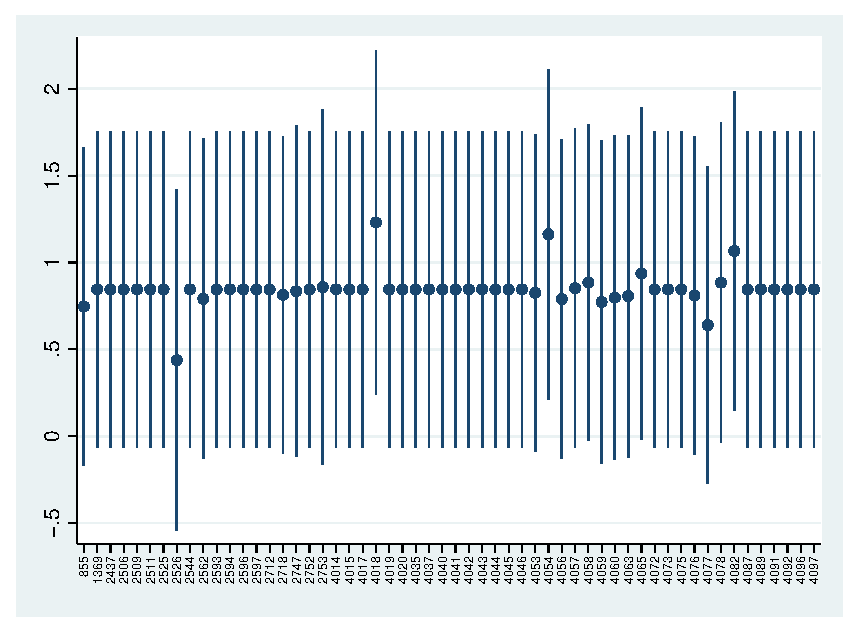
\includegraphics[width=\textwidth]{../../../output/image/coef-interviewer-child-pos_childSDQ_score.eps}       
\caption{Outcome: Positive SDQ Score}        
        \end{subfigure}
        \begin{subfigure}[t]{0.81\textwidth}
          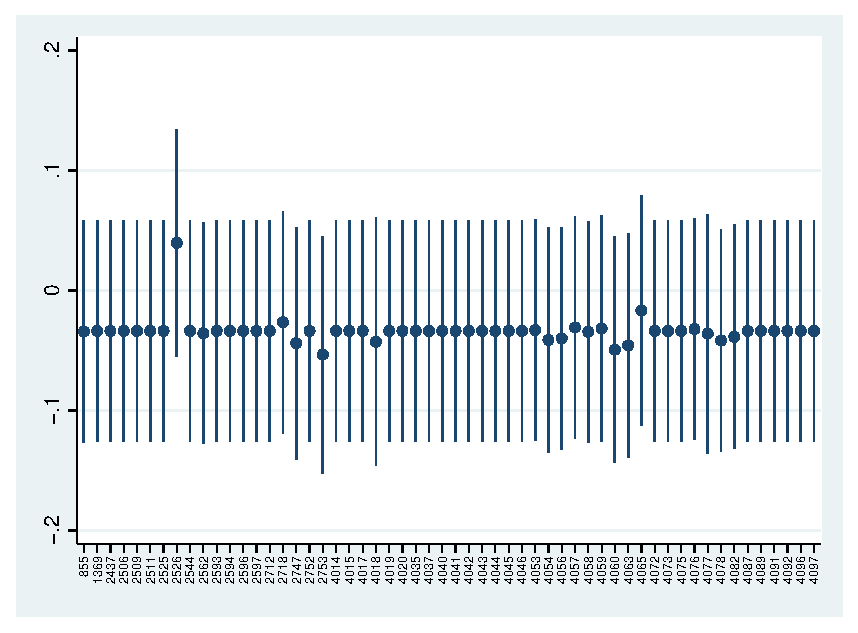
\includegraphics[width=\textwidth]{../../../output/image/coef-interviewer-child-BMI_obese.eps}       
 \caption{Outcome: Not Obese}        
        \end{subfigure}
      \caption{Child Cohort: Droping Each Interviewer}  \label{fig:child-sensitivity-interviewer}
    \end{figure}

    \begin{figure}[H]
      \centering
        \begin{subfigure}[t]{0.81\textwidth}
          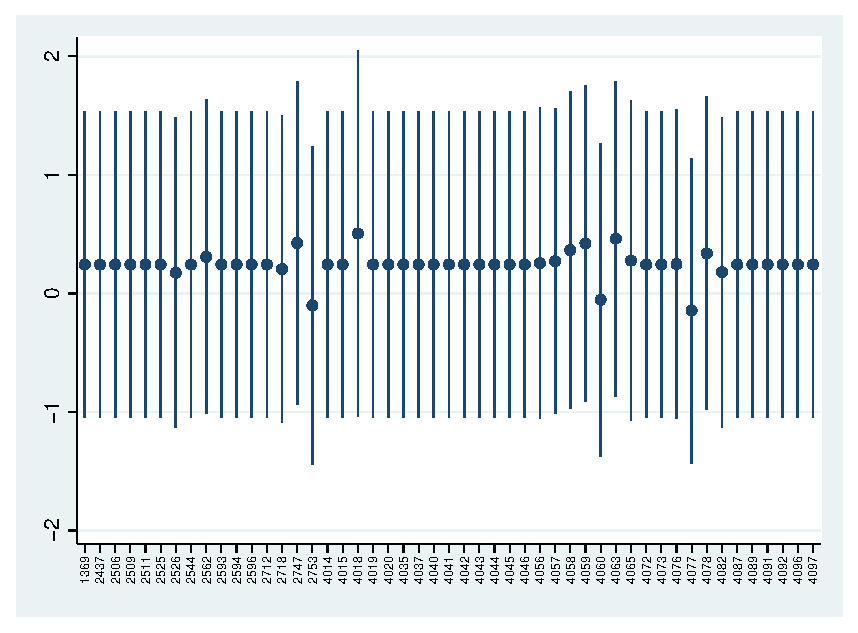
\includegraphics[width=\textwidth]{../../../output/image/coef-interviewer-adol-pos_childSDQ_score.eps}       
\caption{Outcome: Positive SDQ Score}        
        \end{subfigure}
        \begin{subfigure}[t]{0.81\textwidth}
          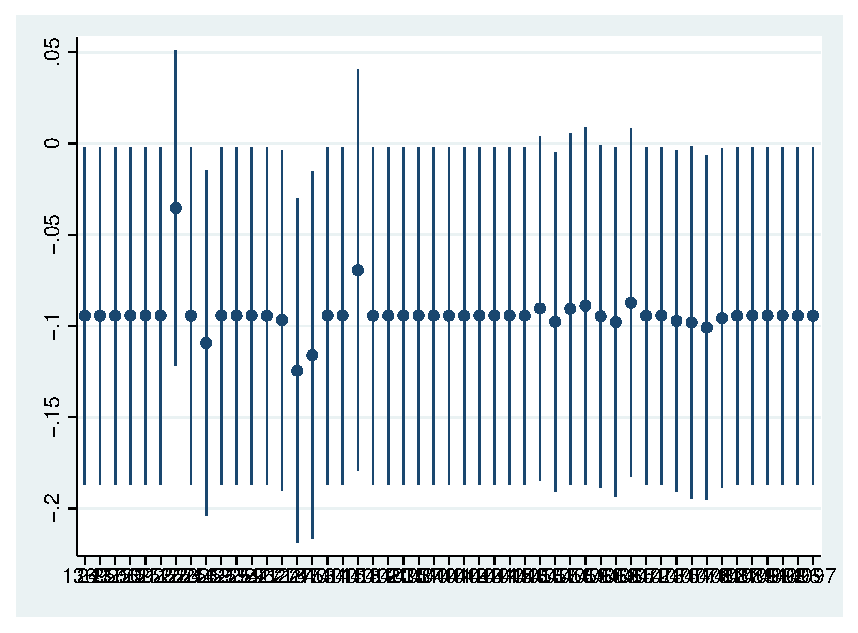
\includegraphics[width=\textwidth]{../../../output/image/coef-interviewer-adol-BMI_obese.eps}       
 \caption{Outcome: Not Obese}        
        \end{subfigure}
      \caption{Adolescent Cohort: Droping Each Interviewer}  \label{fig:adol-sensitivity-interviewer}
    \end{figure}


    \begin{figure}[H]
      \centering
        \begin{subfigure}[t]{0.81\textwidth}
          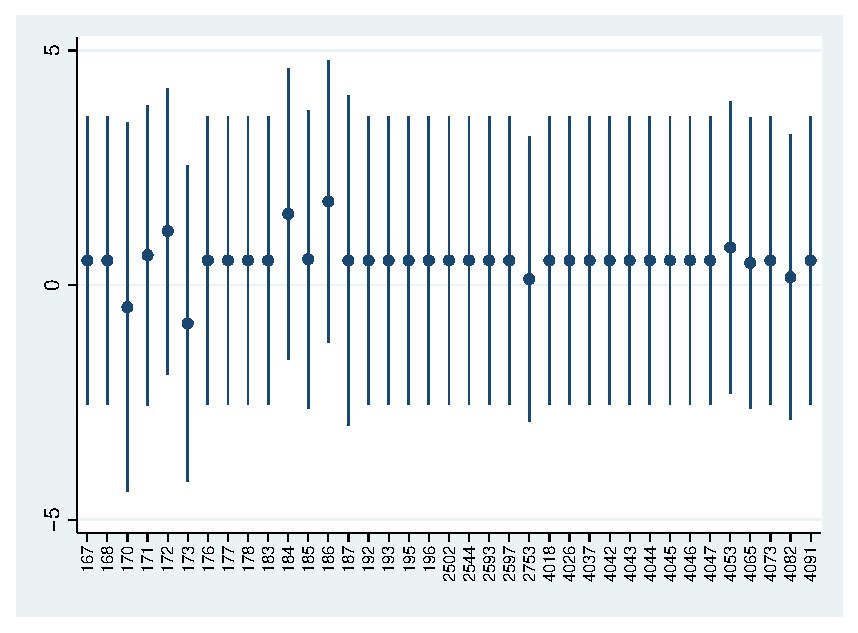
\includegraphics[width=\textwidth]{../../../output/image/coef-interviewer-adult30-votoMaturita.eps}       
\caption{Outcome: Positive SDQ Score}        
        \end{subfigure}
        \begin{subfigure}[t]{0.81\textwidth}
          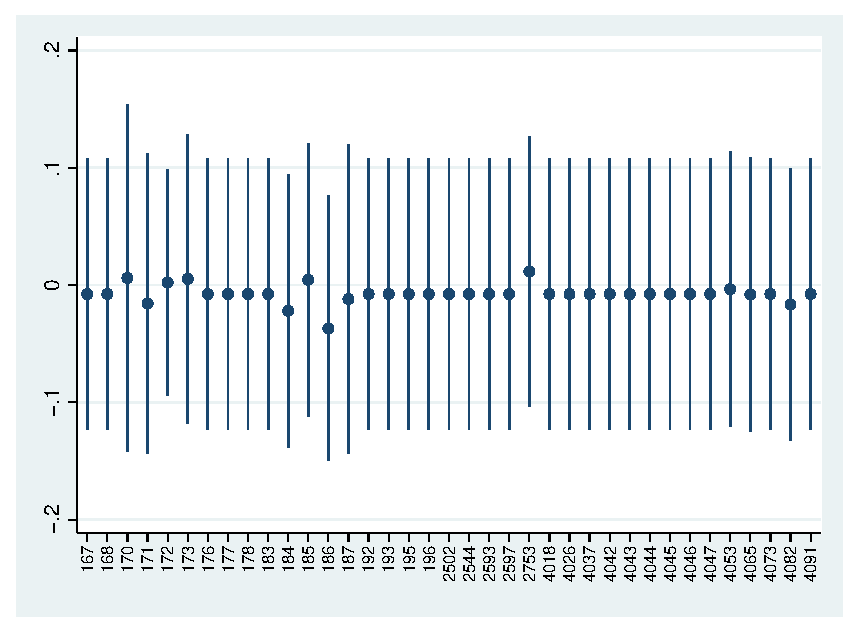
\includegraphics[width=\textwidth]{../../../output/image/coef-interviewer-adult30-BMI_obese.eps}       
 \caption{Outcome: Not Obese}        
        \end{subfigure}
      \caption{Adult-30 Cohort: Droping Each Interviewer}  \label{fig:adult30-sensitivity-interviewer}
    \end{figure}


    \begin{figure}[H]
      \centering
        \begin{subfigure}[t]{0.81\textwidth}
          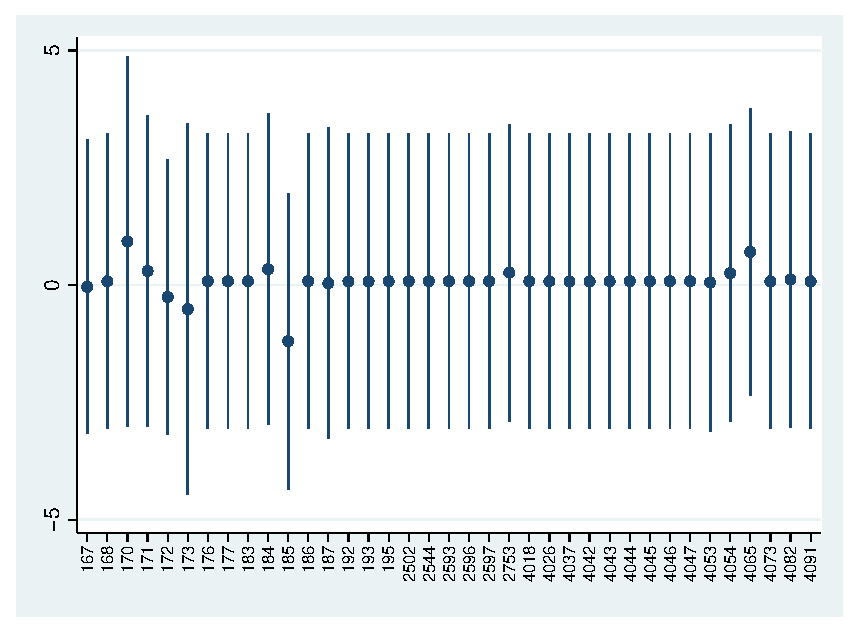
\includegraphics[width=\textwidth]{../../../output/image/coef-interviewer-adult40-votoMaturita.eps}       
\caption{Outcome: Positive SDQ Score}        
        \end{subfigure}
        \begin{subfigure}[t]{0.81\textwidth}
          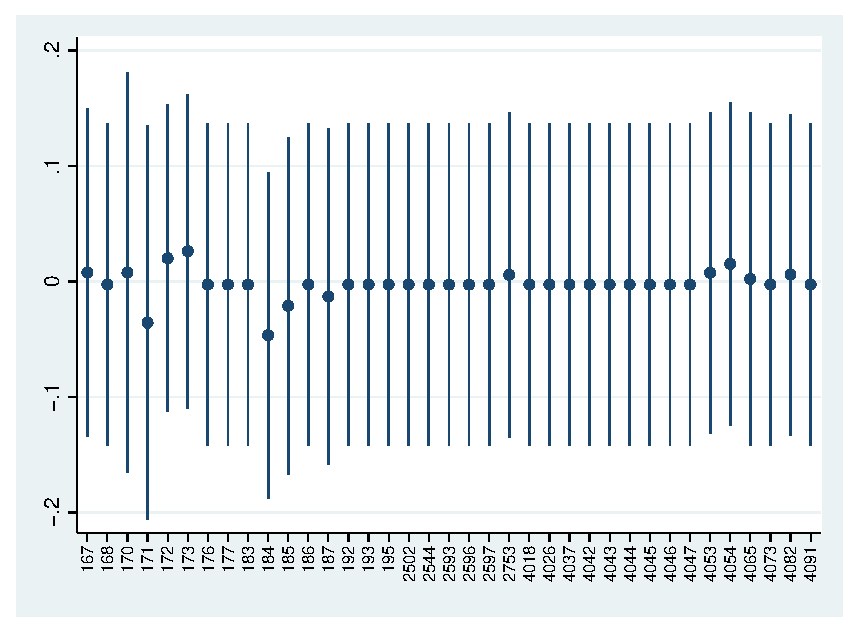
\includegraphics[width=\textwidth]{../../../output/image/coef-interviewer-adult40-BMI_obese.eps}       
 \caption{Outcome: Not Obese}        
        \end{subfigure}
      \caption{Adult-40 Cohort: Droping Each Interviewer}  \label{fig:adult40-sensitivity-interviewer}
    \end{figure}






\end{document}
